\section{Работа со средством}\label{COMMON.Overview}

%%%% Операторы

С~СКЗИ взаимодействуют операторы (см. рис.~\ref{Fig.COMMON.Sessions}).
%
Взаимодействие состоит в вызове сервисов.
%
Сервисы выполняют операции над объектами, используя при этом ресурсы КСК,
при необходимости обращаясь к другим сервисам.
%
С помощью сервисов оператор организует криптографическую
обработку внешних объектов, задействуя объекты СКЗИ.
%
Внутренние функции и механизмы безопасности в основном предназначены
для защиты объектов СКЗИ.

\begin{figure}[bht]
\begin{center}
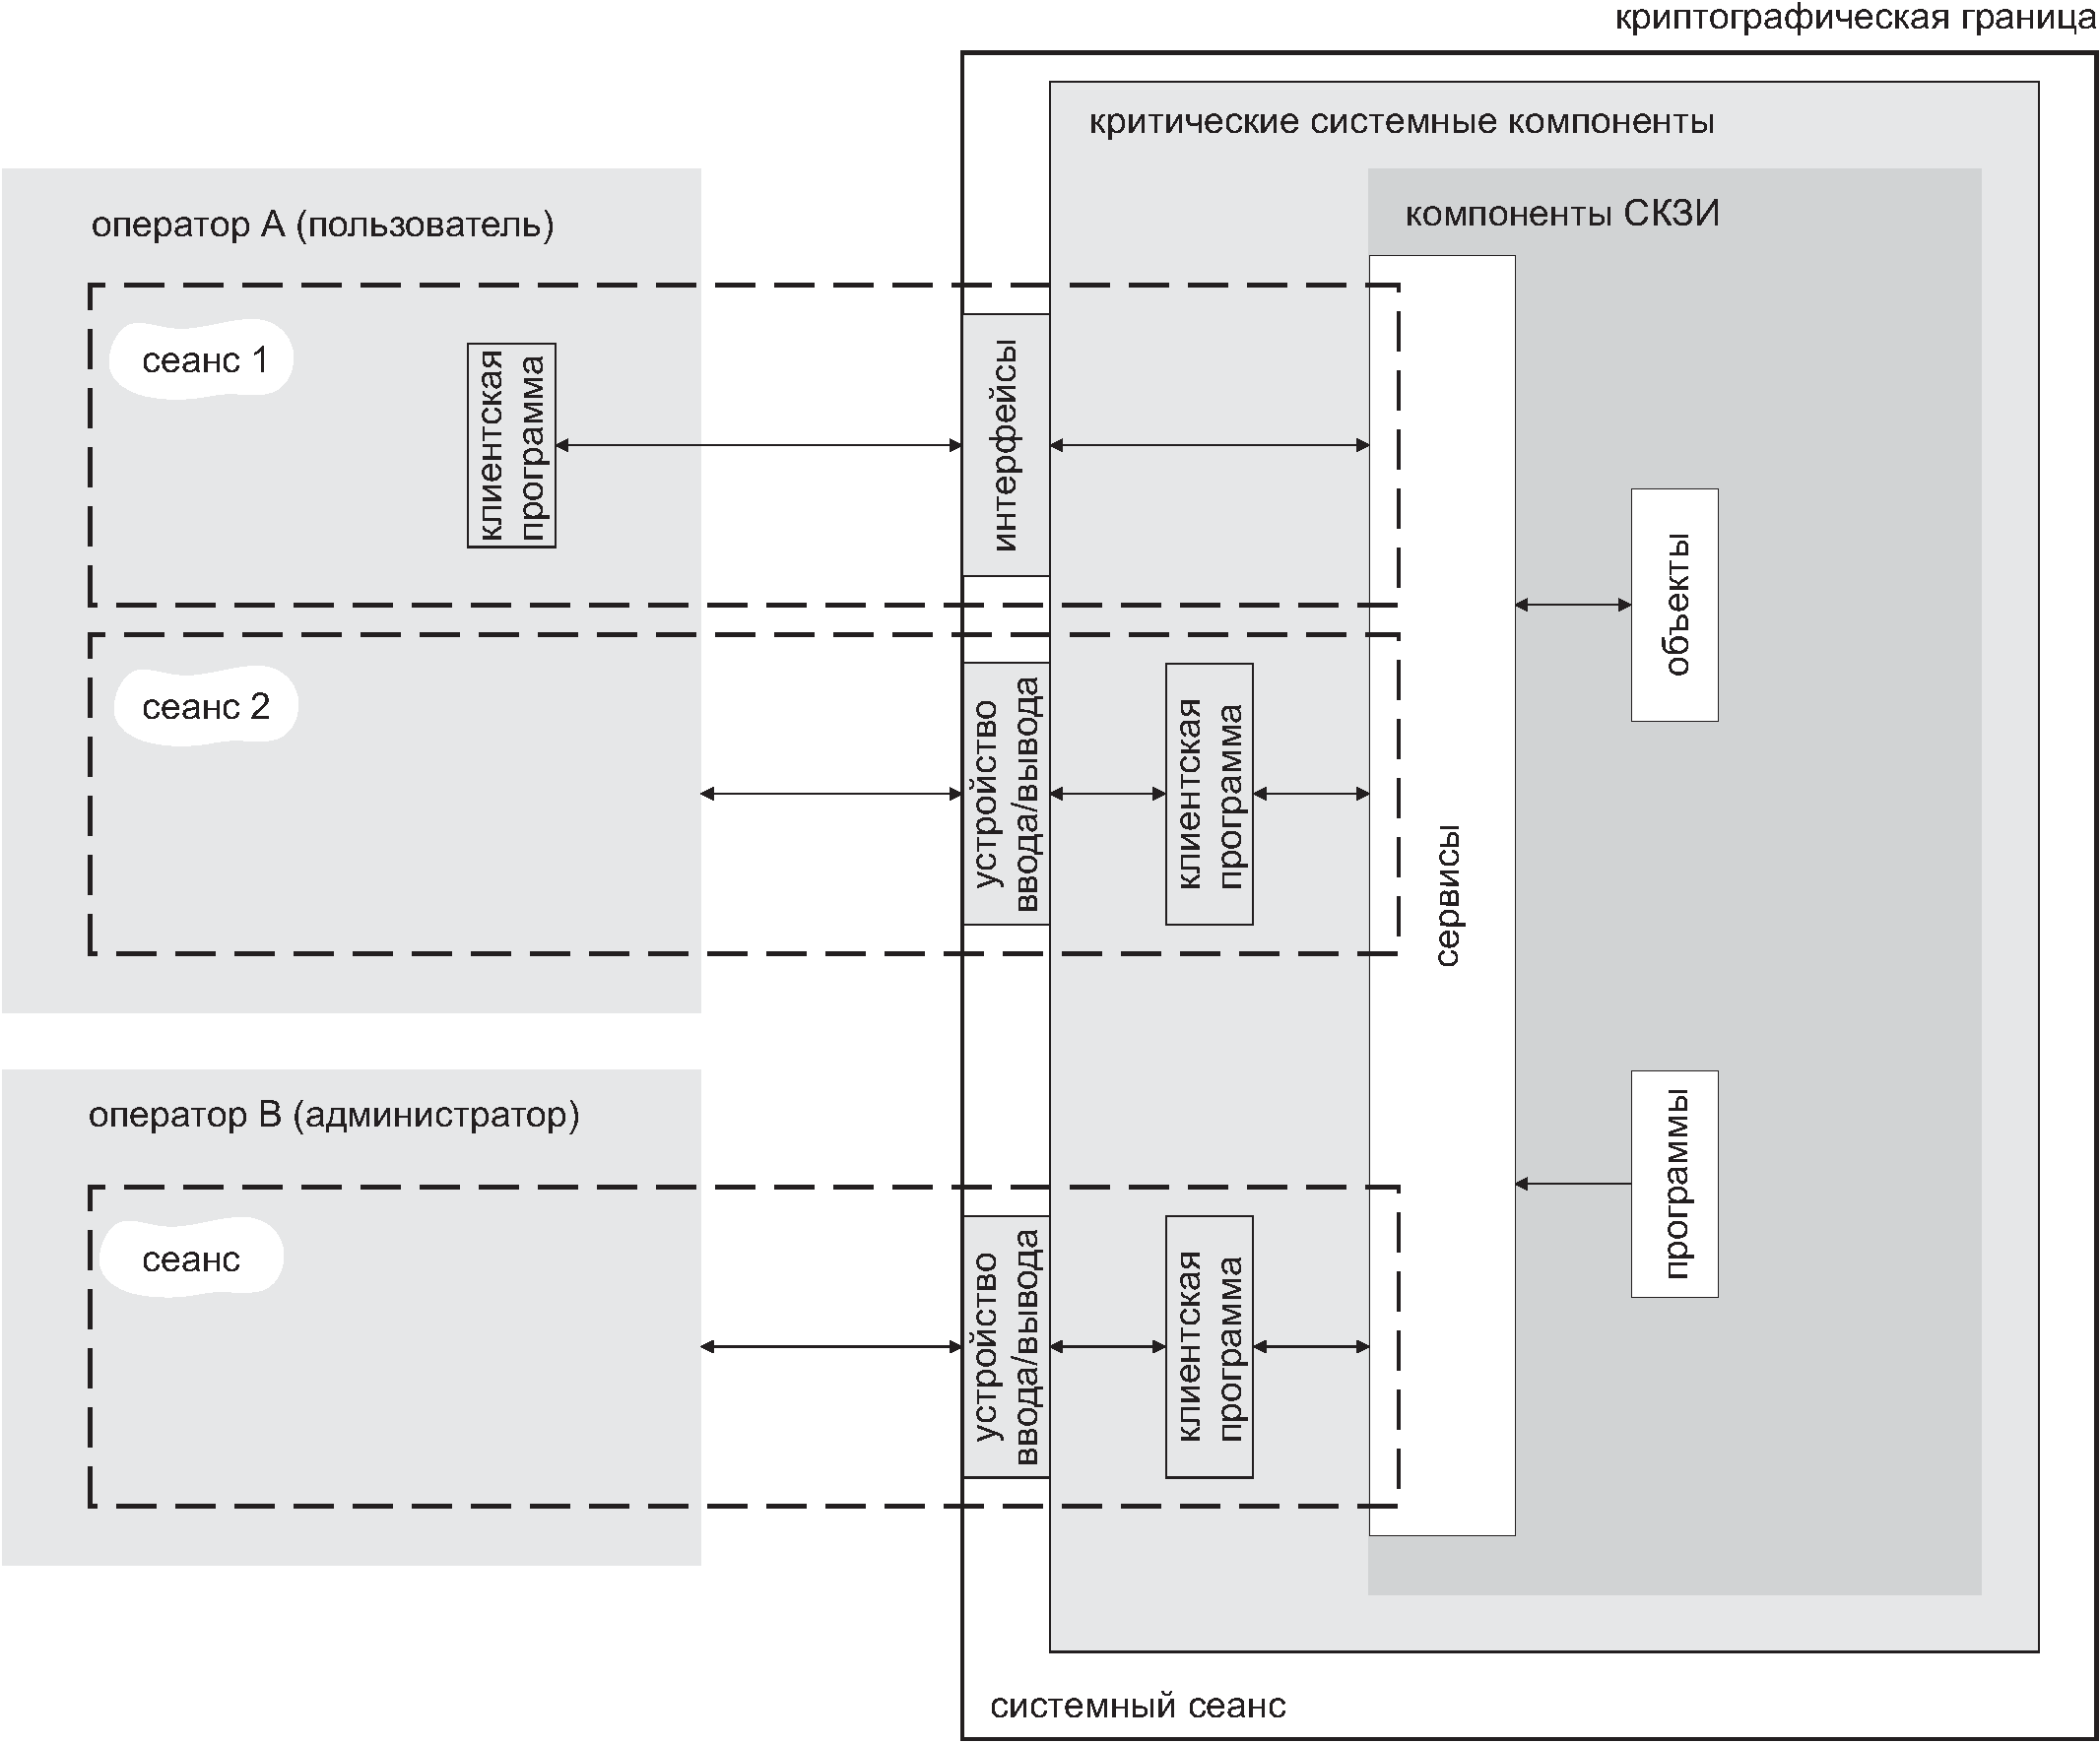
\includegraphics[width=16.5cm]{../figs/sessions}
\end{center}
\caption{Работа со средством}\label{Fig.COMMON.Sessions}
\end{figure}

%%%% Клиентские программы

Оператор взаимодействует с~СКЗИ либо напрямую, 
либо через клиентскую программу: браузер, клиента электронной почты, 
программу электронного документооборота.
%
Клиентская программа может размещаться в системной среде 
или за ее пределами. 
%
В последнем случае канал связи клиентской программы с СКЗИ защищается. 

%%%% Роли

Определены роли (категории) операторов.
%
В~системной среде или в самом СКЗИ реализуются средства аутентификации для
проверки принадлежности оператора к определеной роли и допустимости выполнения
оператором сервисов данной роли.

%%%% Система

Для унификации правил доступа вводится неявный системный оператор.
Он представляет системную среду СКЗИ. Cеанс системного оператора 
(cистемный сеанс) совпадает с непрерывным периодом штатного функционирования 
СКЗИ: от включения (запуска программ) до выключения (завершения).
%
Состояния системного сеанса считаются состояниями самого СКЗИ.

%%%% Общая системная среда

Системная среда может быть общей для нескольких СКЗИ. Эти средства могут 
использовать сервисы друг друга, обмениваться объектами, участвовать в экспорте 
чужих объектов за пределы криптографической границы.

